\subsection{Fairness}
\label{sec:fairness}
%\tanle{organized and shortened this section}

\subsubsection{Existing fair allocations do not work}

When multiple users share the same cluster, fairness is often important in order to provide performance isolation and to avoid starvation. 
In traditional multi-resource allocation problem, where each job has only one configuration, there are four main properties \cite{drf}:

\begin{itemize}
  \item Pareto Efficiency (PE): No user can increase her performance
without hurting the performance of at least another user.

  \item Sharing Incentive (SI): Each user is no worse by sharing
than using $\frac{1}{n}$ of the system resources exclusively.

  \item Envy-Freeness (EF): No user prefers the allocation of another user for better throughput.

  \item Strategy-proofness (SP): No user is able to benefit by lying.

\end{itemize}

% \begin{figure}
% 	\centering
% 	\includegraphics[width=0.7\linewidth]{figs/fairness_ex}
% 	\caption{All CPU cores will remain idle if we allow users to choose their favorite configurations and allocate resource based on DRF. \tanle{this figure is trivial and not referred in the paper --> to be removed.}}
% 	\label{fig:motiv1}
% \end{figure}


DRF \cite{drf} satisfies all four properties when each job has only one configuration. Intuitively, one might expect to extend DRF to the allocation of interchangeable resources. One straightforward extension is to pick the resource configuration with the shortest processing time for each job and then use DRF to allocate the resources by ignoring the interchangeability among resources, e.g., taking CPUs and GPUs as different resource types.
%user estimate their job performance on different resources (CPUs and GPUs), and they demand the resources (one resource from computation and memory) that work the best for that particular job. 
Unfortunately, this does not work. Formally, we have the following lemma regarding this DRF extension.

\begin{restatable}[]{lem}{drf}
	\label{lem:drf_fail}
	If each job picks the configuration with shorter processing time, there exist cases where DRF fails to provide PE, SI or SP under multiple configurations.
\end{restatable}

%\emph{DRF fails to provide SI.}
%However, this approach breaks easily under the simplest setting.
%Assume there are 2 users with identical jobs that prefer GPUs slightly. Both users request GPUs and are allocated half of GPUs, while CPUs are not used. Clearly the sharing incentive is violated as the allocation is worse than equal sharing of all resources between these two users.\mosharaf{Didn't get it.}

Surprisingly, there is a hard tradeoff among these basic properties \cite{sun2018fair}. In particular, we can show for any allocation, if
it provides sharing incentive and Pareto efficiency, it cannot
be strategyproof. Conversely, if it is strategyproof, sharing
incentive and Pareto efficiency cannot be provided simultaneously.
There is one exception: if all jobs have the same speedup by using GPUs, then the problem degenerates to a traditional multi-resource allocation, where DRF can be applied. However, it is not true in practice as shown in Figure~\ref{fig:speedup_rates}. Formally, we have the following impossibility result.

\begin{restatable}[]{lem}{imposs}
\label{lem:imposs}
No multi-configuration allocation can satisfy (i) PE and SI, and (ii) SP simultaneously unless the relative efficiency of CPU and GPU is the same for all jobs. \end{restatable}

%Notice that when relative efficiency of CPU and GPU is the same for all $n$ users, then GPU is equivalent to a faster or slower CPU for all users,  then existing approach can be easily adapted to this case. However, this is not true in reality as shown in Figure \ref{fig:beta}. 

% Interestingly, in current systems, users normally do not know their job characteristics or the system conditions exactly. Therefore, it is hard for users to ``game'' the system. %So strategyproofness seems not necessary.\mosharaf{This doesn't make sense.}
% In addition, we develop an online profiling tool in \name. Therefore, the system no longer requires users to submit their job characteristics.
% %Details can be found in Section ???.
% \mosharaf{ I don't see the point of this discussion.}

% Given the job characteristics estimated by our online profiling tool, another extension of DRF is that: the scheduler sort the jobs based on the relative efficiency on GPUs versus CPUs. 
% Pick a threshold value $b$. If a job's relative efficiency exceeds $b$, pick the GPU configuration. Otherwise, pick the CPU configuration. Then perform DRF by taking CPUs and GPUs as different resource types. 

%The placement will be determined by some fixed threshold value $\beta$, if the efficiency of job $j$ is smaller than $\beta$, it will be placed in CPU, if $j$ is larger than $\beta$, it will be placed in GPU, then the allocation is determined by DRF.


% On the positive side, we have the following result. 

% \begin{restatable}[]{lem}{thresholdDRF} 
% 	\label{lem:thresholdDRF}
% 	If computation is the only bottleneck resource, there exists a threshold-DRF policy that is PE,SI and EF assuming resources are divisible and jobs from the same user are identical.
% \end{restatable}

% However, it is not easy to decide this threshold $b$.
% Especially, when demand changes overtime the threshold is not a constant.
% Moreover, if other resources such as memory can become the bottleneck, any threshold-DRF approach fails to provide desirable properties. More detailed proof is in Appendix \ref{sec:lem:thresholdDRF}
%\mosharaf{I think all these should be relegated to appendix and we should focus on our algorithm.} \tanle{done.}

% Jobs of user $i$ have efficiency 50 while jobs from user $j$ have efficiency 80. The threshold is some value between 50 and 80 so that user $i$'s jobs are placed on CPUs while user $j$'s jobs are placed on GPUs. 
% For jobs of user $i$, assume its CPU configuration is 8 CPU cores and 8 GB memory (we will discuss how to decide the configurations in section ???) and its GPU configuration is 1 GPU and 2 GB memory. Jobs of user $j$ also have GPU configuration with 1 GPU and 2 GB memory. From figure \ref{fig:DRF-threshold}, the allocation is neither SI nor EF. \todo{Why?} \xiao{it is explained in the figure caption, I will update these figures soon using Tan's standard}
% \begin{figure}
% 	\centering
% 	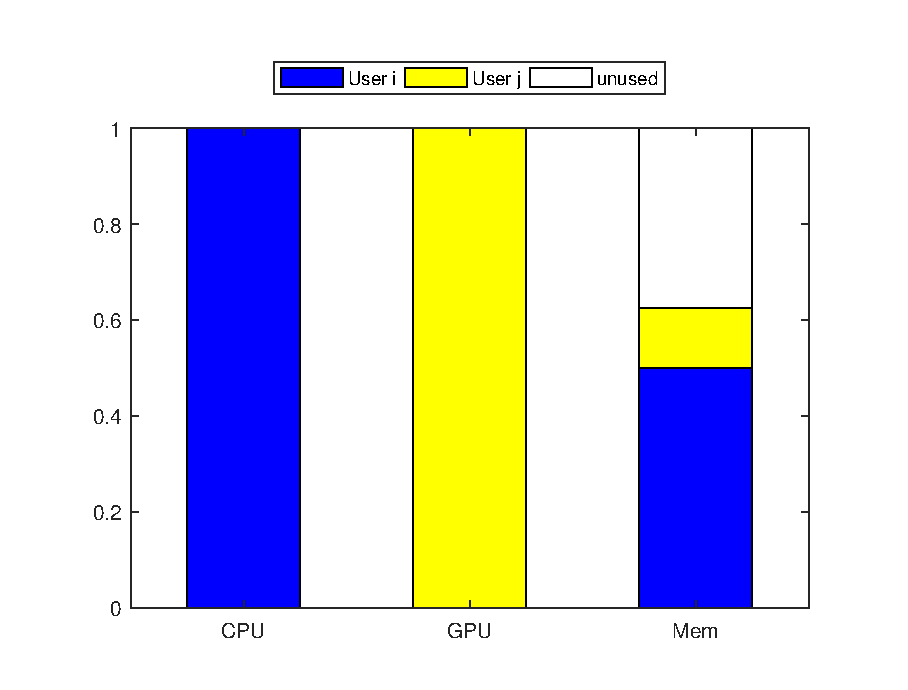
\includegraphics[width=0.8\linewidth]{figs/DRF-threshold}
% 	\caption{All CPU cores belongs to User $i$ based on DRF. The allocation is still worse than equal sharing for User $i$ as 128 CPU cores worth less than 4 GPUs for User $i$. }
% 	\label{fig:DRF-threshold}
% \end{figure}


% \begin{figure}
% 	\centering
% \includegraphics[width=0.8\linewidth]{figs/DRF-merge}
% 	\caption{All CPU cores belongs to User $i$ based on DRF. The allocation is still worse than equal sharing for User $i$ as 128 CPU cores worth less than 4 GPUs for User $i$. }
% 	\label{fig:DRF-merge}
% \end{figure}

\subsubsection{Our idea}
\label{sec:fairness_score}

\name maintains a progress for each user over time. Whenever a resource becomes available, \name schedules jobs from users with lower progress for fairness. The key is therefore how to update the progress measure over time.  
For job $i$, it has the CPU configuration $(c, m_c, p_c)$, where $c$ is the CPU demand, $m_c$ is the memory demand, and $p_c$ is the processing time on CPU, and the GPU configuration $(g, m_g, p_g)$, where $g$ is the GPU demand, $m_g$ is the memory demand, and $p_g$ is the processing time on GPU. 

If $p_c$ is smaller than $p_g$ (CPU is more effective), we use the dominant share of the CPU configuration $d_i=\max\{c/C, m_c/M\}$, where $C$ and $M$ are the CPU and memory capacity of the cluster. 
Otherwise, we use the dominant share of the GPU configuration $d_i=\max\{g/G, m_c/M\}$, where $G$ is the GPU capacity of the cluster. 

The (instantaneous) value of the job $i$ is based on the dominant share, but discounted if the job is not placed on the more effective resource. For instance, if job $i$ is more effective on GPU but is placed on CPU, its value $v_i = \frac{p_g}{p_c} d_i = \frac{p_g}{p_c} \max\{g/G, m_g/M\}$. A user's progress is the sum of values of all her jobs that are currently running.

%We define the progress of a user based on instantaneous dominant share.  
% The idea is the following: Every user wishes his/her jobs to be finished as fast as possible. But sometimes, that is not doable as some jobs have to sacrifice and take the suboptimal configurations for the performance of other jobs. The system shouldn't punish them for taking a suboptimal solution and finish slower.\mosharaf{Unclear what it means.} For example, assume a job can finish within 5 mins on GPU or 20 mins on CPU, the CPU unit time/score of the job should be $\frac{1}{4}$ of the GPU counterpart.

% \xiao{I rewrote above paragraph}

%The idea is the following: 
% As each job has two configurations with different processing times.  From users perspective, they all prefer to pick the configuration that results in a better completion time. However, this is not always possible, as there might be intense competitions among users from their favorite resource in a cluster. As a consequence, some jobs have to sacrifice and take the suboptimal configurations for discounted progress. For example, assume a job can finish within 5 mins on GPU or 20 mins on CPU, the CPU unit time/progress of the job is $\frac{1}{4}$ of the GPU counterpart.




% score $v(i)$ for a single job $i$ will be calculated only when the job is being processed.

% From the configuration matrix $$
% Q_i=
% \begin{bmatrix}
% c_i & m_i^1 & p_i^1 \\
% g_i & m_i^2 & p_i^2 
% \end{bmatrix} $$

% Let the faster configuration in the matrix be $(x_i,m_i,p_i)$. Let the dominant share of this configuration be $d_i$, where
% \[
% d_i=
% \begin{cases}
% \max(\frac{x_i}{C_1},\frac{m_i}{C_3}), & p_i^1 \leq p_i^2 \\
% \max(\frac{x_i}{C_2},\frac{m_i}{C_3}), & p_i^1 > p_i^2
% \end{cases}
% \]


% Then

% \[
% v_i=
% \begin{cases}
% \frac{p_i}{p^1_i}d_i, & \mbox{If job $i$ placed on CPU} \\
% \frac{p_i}{p^2_i}d_i, & \mbox{If job $i$ placed on GPU}
% \end{cases}
% \]


% % simply compare $p_i^1$ and $p_i^2$ and check the placement of job $i$. \begin{itemize}
% % 	\item If $p_i^1 <  p_i^2$, and job $i$ is placed on CPU, then $v(i) = \max(\frac{c_i}{C_1},\frac{m_i^1}{C_3})$;
% % 	\item If $p_i^1 <  p_i^2$, and job $i$ is placed on GPU, then $v(i) = \frac{p_i^1}{p_i^2}\max(\frac{c_i}{C_1},\frac{m_i^1}{C_3})$;
% % 	\item If $p_i^1 \geq  p_i^2$, and job $i$ is placed on CPU, then $v(i) = \frac{p_i^2}{p_i^1} \max(\frac{g_i}{C_2},\frac{m_i^2}{C_3})$;
% % 	\item If $p_i^1 \geq  p_i^2$, and job $i$ is placed on GPU, then $v(i) = \max(\frac{g_i}{C_2},\frac{m_i^2}{C_3})$;
% % \end{itemize} 



% Where $(C_1,C_2,C_3)$ represents the cluster capacity of \\$(CPU,GPU,MEM)$.
% The progress of a user is the sum of all scores from its jobs that are currently being processed. 

%\todo{add explanations}

%The score is a composition of two parts: the preferred configuration, and actual configuration from scheduling. The former decides the dominant share of the job, while the latter decide the scaling of the dominant share

Consider a simple example where the job has CPU configuration $(1, 4, 20)$ and GPU configuration $(1, 2, 5)$. The system capacity is $(8, 2, 64)$ for CPU, GPU, and memory. 
Because GPU provides a shorter processing time, the dominant share of the job is $\frac{1}{2}$. If the job is actually scheduled on GPU, its value is $\frac{1}{2}$. Otherwise it is discounted by $\frac{1}{4}$ ( to $\frac{1}{8}$) because running on CPU is 4 times slower than GPU. 

Generally speaking, the value of a job is decided by its preferred configuration and the actually resource allocated to it. The former decides the dominant share of the job similar to DRF using the preferred configuration, while the latter decides the speed of consuming that dominant share. In our example, as the job will run 4 times longer on CPU, its (instantaneous) value is divided by 4. Over the execution of the job, either on CPU or GPU, its aggregated value is the same. 
Actually, the progress of a user can be viewed as her instantaneous throughput. %For the example above, and assume the system has 2 identical users. When the progress of two users equal, then either they share both CPU and GPU (i.e, each get 4 CPUs and 1 GPU) or one gets all CPUs and 0 GPU while the other get 2 GPUs. In any case, the throughput speeds of for both users are 2 ($1+\frac{1}{4}\times 4 = \frac{1}{4}\times 8 +0 = 0+2)$.




% $$Q_1 =
% \begin{bmatrix}
% 4 & 4 & 20 \\
% 1 & 4 & 5  \\ 
% \end{bmatrix} $$
% with cluster capacity $(20,10,50)$. Clearly, user prefer GPU as the GPU configuration is 4 times faster than CPU. The dominant share of the job is thus $\frac{1}{10}$. If the job is eventually scheduled on GPU, then the score is also $\frac{1}{10}$; if it is on CPU instead, the score is $\frac{1}{40}$.

% To understand above
% As each job has two configurations with different processing times.  From users perspective, they all prefer to pick the configuration that results in a better completion time. However, this is not always possible, as there might be intense competitions among users from their favorite resource in a cluster. As a consequence, some jobs have to sacrifice and take the suboptimal configurations for discounted progress. For example, assume a job can finish within 5 mins on GPU or 20 mins on CPU, the CPU unit time/progress of the job is $\frac{1}{4}$ of the GPU counterpart.




% Actually, we can prove the following: 

% \begin{restatable}[]{lem}{imposs}  If the progress of all users equal, then the allocation is envy-free, moreover, if either computation or memory is used up, the allocation is Pareto-efficient and sharing-incentive.\end{restatable}

% The intuition behind the lemma is that the progress is a way to measure 'effective resource' a user receive, if the score is same for all users, then they are treated equally by the system.

\subsubsection{Incorporating fairness into \name}

%Given the fairness system we designed in section 4.2, we can use the progress to evaluate how much resource is being used by a user at the current time. Then clearly we should prioritize users with lower progress.

\name provides a fairness knob and the system operator can adjust its value $\alpha$ in $[0,1]$, which affects how many users are taken into consideration when a scheduling is triggered. For instance, with 20 users and $\alpha = 0.3$, only jobs from 6 users with lowest progress are considered for scheduling. When $\alpha=1$, there is no fairness constraint and all users are considered. The \name algorithm is based on Algorithm~\ref{alg:greedy} and incorporates online arrivals and fairness considerations. 

%\todo{Add the Allox algorithm formal description with fairness consideration}
%\xiao{I edited the algorithm as the following with some extra explanations}
\begin{algorithm}[H]
\small
\caption{\name Scheduler}
\label{alg:allox_scheduler}
\begin{algorithmic}[1]
	\Function{ScheduleNextJob}{available machine $i$}
    \State {Update users' progress and get the set of users $A_{\alpha}$ consisted of $\ceil*{\alpha n}$ users with the lowest progress.} %whose fairness score is within $\ceil*{\alpha n}$ of all users}
    \ForAll{job $j$ in the waiting queue from $A_{\alpha}$}
    \State Add processing time of job $j$ to matrix $P$
    \EndFor
    \State Generate the delay matrix $D$ and further the cost matrix $Q$;
    %\State Generate cost matrix $Q$ using  equation \ref{eq:generate_cost}
    \State Solve the min-cost matching problem defined by $Q$ to get the matching matrix $M$
    \For{$k = J:1$ } \Comment{$J$ is the total \# of jobs in $A_{\alpha}$}
      \For {$w = 1:J$}
        \If{$M(w,m(k-1)+i) = 1$} \Comment{$w$ is first job scheduled on machine $i$}
          \State schedule job $w$ to machine $i$
          \State Update available time $\omega_i$ and users' progress
          %\State Update users' progress %$v_{j \in u}(u)$
          \State \Return job $w$
      % 	\State Break
        \EndIf
      \EndFor
    \EndFor
	\State \Return null
    \EndFunction
%     \State Generate matrix $Q$;
%     \State Solve a min-cost bipartite matching problem for matrix $Q$;
%     \State Retrieve scheduling from the solution
\end{algorithmic}
\end{algorithm}
%\xiao{ new explanations}

Lines 2-6 of Algorithm~\ref{alg:allox_scheduler} are preparing the input for the matching problem. In particular, it only considers jobs from $\ceil*{\alpha n}$ users with the lowest progress. 
After solving the min-cost matching problem in Line 7, the algorithm simply searches for the first job scheduled on machine $i$. 
%In the above scheduling part (line 8-18), the solver for matching problem is the same as in Algorithm 1, but when the scheduler gets the matching matrix $M$, it only schedules 1 job. 
Specifically, the scheduler checks all entries affiliated with the available machine $i$ and find a valid entry with largest $k$, which implies that the corresponding job $w$ is scheduled first according on machine $i$. Recall that $k$ represents the last $k$-th job on a machine. Therefore, the larger $k$ is, the earlier the job is scheduled on that machine.

Occasionally, the scheduler cannot find a valid job. It occurs when no job is scheduled on the available machine based on current jobs and system load. Consider a simple example with 2 jobs, both have 1 minute processing time on GPUs and 10 minutes processing time on CPUs. Assume the cluster has only 1 CPU and 1 GPU. After the scheduler places any job on the GPU, even though the CPU is available, the optimal schedule for the other job is to wait. In this case, the algorithm returns no job and the system waits until the next event such as new job arrivals or a new machine becomes available. For instance, with no new jobs, after 1 minute, the GPU becomes available, and the remaining job will be scheduled on the GPU.




